\graphicspath{ {Figures/interoperability/} }
\chapter{Διασυνδεσιμότητα}\label{ch:Interoperability}
\section{Απαιτήσεις}

\section{Πρωτόκολλα επικοινωνίας}
	\subsection{HL7 messaging v2 και v3}

	\subsection{CDA Documents}
	

		
\section{Δυνατότητες διασύνδεσης με άλλα υποσυστήματα}

	\subsection{Ηλεκτρονική Συνταγογράφηση}
	
		Η διαδικασία της συνταγογράφησης φαρμάκων μπορεί να είναι ιδιαίτερα περίπλοκη και επιρρεπής σε λάθη, με
δυσμενείς επιπτώσεις για την ασφάλεια των ασθενών. Η πρόληψη των επιπλοκών που μπορούν να προκύψουν λόγω ακατάλληλης συνταγογράφησης είναι μία πρόκληση που αντιμετωπίζει το σύστημα υγείας σε παγκόσμιο επίπεδο. Οι λανθασμένες φαρμακευτικές αγωγές, οι παρενέργειες των φαρμάκων και η αποτυχία σωστής συνταγογράφησης που να συντελέσει στην θεραπεία του ασθενούς εκτός του γεγονότος ότι αποτελεί απειλή για την ασφάλεια του, οδηγεί σε σημαντικές δαπάνες για τα συστήματα υγειονομική περίθαλψης. Οι πληροφορίες σχετικά με το ιστορικό του ασθενούς, τις αλλεργίες, τις παρελθοντικές και τις τρέχουσες φαρμακευτικές αγωγές καθώς και τα εργαστηριακά αποτελέσματα του είναι άκρως απαραίτητα ώστε οι κλινικοί ιατροί να συνταγογραφήσουν την κατάλληλη φαρμακευτική αγωγή, αλλά είναι συχνά δεν είναι διαθέσιμα. \cite{prescribingErrors} Στην Ελλάδα ειδικότερα, υφίσταται το πρόβλημα της αλόγιστης ή πλασματικής συνταγογράφησης με αποτέλεσμα να  χρειάζονται μέτρα για την επαναφορά της αξιοπιστίας της διαδικασίας.  Χαρακτηριστικό παράδειγμα είναι τα στοιχεία του Υπουργείου Υγείας και Κοινωνικής Ασφάλισης, με βάση τα οποία το έτος 2009 εκτελεστήκαν στην Ελλάδα περίπου 100 εκατομμύρια ετησίως ενώ αντίστοιχα στην Δανία εκτελέστηκαν μόνο 15 εκατομμύρια συνταγές.


		Με τον όρο ηλεκτρονική συνταγογράφηση (e-prescription) σύμφωνα με το Εθνικό Σύστημα Υγείας στην Αγγλία αναφερόμαστε στην αξιοποίηση των ηλεκτρονικών συστημάτων για την διευκόλυνση και την ενίσχυσης της επικοινωνίας μίας ιατρικής εντολής ή συνταγής, βοηθώντας στην επιλογή, τη διαχείριση και την προμήθεια ενός φαρμάκου μέσω της γνώσης και υποστήριξης αποφάσεων, παρέχοντας μια διαδρομή ελέγχου για το σύνολο της διαδικασίας χρήσης των φαρμάκων.  Τα συστήματα ηλεκτρονικής συνταγογράφησης που προσφέρουν ηλεκτρονική υποστήριξη στους κλινικούς ιατρούς έχουν σχεδιαστεί για να βοηθήσουν στην περίπλοκη διαδικασία της συνταγογράφησης. \cite{Kierkegaard2013} Επιτρέπουν σε έναν γιατρό, έναν φαρμακοποιό, μία νοσηλεύτρια να διαβιβάσει χωρίς σφάλματα, ακριβείς και κατανοητές συνταγές ηλεκτρονικά, μέσα από τον φορέα παροχής υπηρεσιών υγείας, στο φαρμακείο.  \cite{eprescr}
		
		
		Τα συστήματα ηλεκτρονικής συνταγογράφησης μπορεί να έχουν λειτουργικές δυνατότητες για την παροχή βασικής υποστήριξης αποφάσεων, όπως ο έλεγχος για τυχόν αλλεργίες στα φάρμακα, βασικές κατευθυντήριες γραμμές για τη δοσολογία, τεστ για πιθανές αντιδράσεις μεταξύ φαρμάκων κ.λ.π. Τα συστήματα αυτά είναι ιδιαίτερα χρήσιμα στο τεχνικό κομμάτι της συνταγογράφησης κατάλληλων φαρμάκων, καθώς προσφέρουν λειτουργίες όπως ο υπολογισμός της σωστής δόσης ή ο εντοπισμός αλληλεπιδράσεων μεταξύ των φαρμάκων. \cite{Kart2008}

		Τα συστήματα ηλεκτρονικής συνταγογράφησης χωρίζονται σε δύο κατηγορίες:
		
		\begin{itemize}
		
		\item Τα αυτόνομα συστήματα (stand alone systems). Πρόκειται για λειτουργικά συστήματα τα οποία είναι εγκατεστημένα στους ηλεκτρονικούς υπολογιστές  και χρησιμοποιούνται είτε αυτόνομα είτε μέσω σύνδεσης στο διαδίκτυο.  Τα συστήματα αυτά χρησιμοποιούνται κυρίως για τον έλεγχο θεμάτων ασφάλειας και γίνεται προσπάθεια αντικατάστασης τους από τα ολοκληρωμένα συστήματα συνταγογράφησης.

		\item Τα ολοκληρωμένα συστήματα συνταγογράφησης (Electronic Health Record, EHR Systems). Στα συστήματα αυτά ο ιατρός έχει στην διάθεση του όλο το ιστορικό του ασθενούς, τα αποτελέσματα των εξετάσεων του και τα χρησιμοποιεί για να βοηθηθεί στην επιλογή της κατάλληλης δραστικής ουσίας. Οι συναγερμοί ασφαλείας στην περίπτωση αυτή είναι πιο εξειδικευμένοι και ακριβείς.  

		\end{itemize}
		

		Συνοπτικά τα συστατικά της ηλεκτρονικής συνταγογράφησης μπορούν να κατηγοριοποιηθούν σε βασικές δυνατότητες συνταγογράφησης, πληροφορίες για το πλάνο υγείας και τις κλινικές ειδοποιήσεις (clinical alerts).  Οι δυνατότητες συνταγογράφησης περιλαμβάνουν μια λίστα φαρμάκων, οδηγίες για τους ασθενείς, τον αριθμός των εγκεκριμένων ποσοτήτων, σχόλια του γιατρού που συνταγογραφεί προς τον φαρμακοποιό, καθώς και το πεδίο PRN. Οι πληροφορίες για το πλάνο υγείας του ασθενούς περιλαμβάνουν την ιατρική ασφάλεια που έχει και το ιστορικό των φαρμακευτικών αγωγών. Τέλος, οι κλινικές ειδοποιήσεις  βασίζονται στα δημογραφικά στοιχεία και στα στοιχεία του ιατρικού ιστορικού του ασθενούς και περιλαμβάνουν τις αντιδράσεις μεταξύ των φαρμάκων, τις αλλεργίες, τις προειδοποιήσεις για συγκεκριμένες ηλικιακές ομάδες και την κατάλληλη προσαρμογή της δόσης με βάση το βάρος του ασθενούς. \cite{prescribing} 
		
		
		Τα βασικά συστατικά ενός συστήματος ηλεκτρονικής συνταγογράφησης είναι \cite{Grossman2012}:

		\begin{itemize}

		\item Ο παραπέμπων ιατρός. Ο θεράπων ιατρός είναι ο κύριος χρήστης  του συστήματος. Για την σύνδεση του στο σύστημα ακολουθείται μιας διαδικασία επαλήθευσης ώστε να επιβεβαιωθεί η ταυτότητά του. 
Οι αναζητήσεις του θεράποντα ιατρού στην βάσης δεδομένων που περιέχει τους φακέλους των ασθενών πραγματοποιείται με τη χρήση ειδικών πληροφοριών για τον ασθενή, συνήθως το ΑΜΚΑ για Ελλάδα ή τον αριθμό κοινωνικής ασφάλισης (social security number) στον εξωτερικό. Μόλις προσπελαστεί το σωστό αρχείο του ασθενούς, ο ιατρός εξετάζει τις ιατρικές πληροφορίες που περιέχει και προσθέτει ή ενημερώνει μία συνταγή στον ιατρικό φάκελο.
		
		\item Ο κόμβος συναλλαγών. Αποτελεί τον κοινό σύνδεσμο μεταξύ όλων των φορέων (παραπέμπων ιατρός και φαρμακείο). Αποθηκεύει και διατηρεί ένα κύριο κατάλογο των ασθενών για να υπάρχει η δυνατότητα γρήγορης πρόσβασης στις ιατρικές πληροφορίες των ασθενών, καθώς και στην λίστα των φαρμακείων. Όταν ο παραπέμπων ιατρός ανεβάσει κάποια νέα συνταγή στον φάκελο του ασθενούς, τότε αυτή μεταφέρεται αυτόματα και στον κόμβο συναλλαγών. Ο κόμβος συναλλαγών θα στείλει αυτόματα τις πληροφορίες  με στο κεντρικό σύστημα διαχείρισης το οποίο θα απαντήσει με πληροφορίες σχετικά με την καταλληλότητα του ασθενή και το ιστορικό των φαρμακευτικών αγωγών του.  Ο κόμβος συναλλαγών έπειτα στέλνει τις πληροφορίες στον ιατρό έτσι ώστε να έχει τις απαραίτητες πληροφορίες που του χρειάζονται και να ολοκληρώσει και να εγκρίνει την συνταγή. 
		
		\item Το κεντρικό σύστημα διαχείρισης δεδομένων, στο οποίο βρίσκονται όλα τα στοιχεία ιατρικού φακέλου που ελέγχει την καταλληλότητα του ασθενή καθώς και της συνταγής. Το κεντρικό σύστημα διαχείρισης δεδομένων επικοινώνει με τον ιατρό και το φαρμακείο.
		
		\item Το φαρμακείο που έχει εγκατεστημένο το λογισμικό της ηλεκτρονικής συνταγογράφησης. Το φαρμακείο ανακτά την συνταγή από  το κεντρικό σύστημα διαχείρισης συναλλαγών μέσω του κόμβου συναλλαγών και έχει επιπλέον την ικανότητα να επικοινωνήσει με τον ιατρό και να τον ενημερώσει ότι η παραγγελία εκτελέστηκε. 
		
		\end{itemize}
		
		
		
		\subsubsection{Ηλεκτρονική Συνταγογράφηση στην Ελλάδα}
		
		Η ηλεκτρονική συνταγογράφηση στην Ελλάδα βασίζεται στις οδηγίες του νόμου 3892/2010 (ΦΕΚ 189 Α) «Ηλεκτρονική καταχώριση και εκτέλεση ιατρικών συνταγών και παραπεμπτικών ιατρικών εξετάσεων». Σε αυτόν το νόμο καταγράφονται τα ζητήματα ηλεκτρονικής συνταγογράφησης και τα ζητήματα των ηλεκτρονικών παραπεμπτικών.
		
		Ο υπεύθυνος φορέας στην Ελλάδα είναι η Γενική Γραμματεία Κοινωνικών Ασφαλίσεων του Υπουργείου Εργασίας, Κοινωνικής Ασφάλισης και Πρόνοιας. Το σύστημα υποστηρίζεται ηλεκτρονικά από την Ηλεκτρονική Διακυβέρνηση Κοινωνικής Ασφάλισης (ΗΔΙΚΑ Α.Ε.). Η ΗΔΙΚΑ αποτελεί μια ανώνυμη, μη κερδοσκοπικού χαρακτήρα του δημοσίου την οποία αποζημιώνουν οι εξυπηρετούμενοι φορείς για τις υπηρεσίες του παρέχει, όπως για παράδειγμα το έργο μισθοδοσίας των φορέων.  \cite{idika}
		
		Με τον όρο ηλεκτρονική συνταγογράφηση αναφερόμαστε στη παραγωγή, στην διακίνηση και στον έλεγχο των ιατρικών συνταγών και των παραπεμπτικών για ιατρικές πράξεις, με τη χρήση τεχνολογίας ηλεκτρονικών υπολογιστών και επικοινωνιών, έτσι ώστε να διασφαλίζεται η ασφάλεια, η εγκυρότητα και η διαφάνεια στις πληροφορίες που διακινούνται. Ουσιαστικά, το σύστημα περιλαμβάνει ένα αριθμό από διαδικασίες που σχετίζονται με τη δημιουργία, την εκτέλεση, τη διαχείριση, τον έλεγχο, την εκκαθάριση και την εξόφληση μιας φαρμακευτικής συνταγής ή ενός παραπεμπτικού για ιατρικές πράξεις. Διέπει όλα τα συστήματα και τις τοποθεσίες που εμπλέκονται όπως τα τακτικά ιατρεία των νοσοκομείων ή τα ιδιωτικά ιατρεία, τα κέντρα υγείας, τις κλινικές, τα διαγνωστικά κέντρα, τα φαρμακεία και τα ασφαλιστικά ταμεία.


		
		Το ολοκληρωμένο σύστημα ηλεκτρονικής συνταγογράφησης στην Ελλάδα εξυπηρετεί τους εξής σκοπούς:
		
		\begin{itemize}

		\item  Βοηθά στον αποτελεσματικό εκσυγχρονισμό του συστήματος της φαρμακευτικής περίθαλψης. Οι χειρόγραφες συνταγές έχουν αντικατασταθεί από τις ηλεκτρονικές και η διαδικασία έχει αυτοματοποιηθεί.
		 
		\item Συντελεί στην ταυτοποίηση και τον έλεγχο των εμπλεκομένων για να διασφαλίσει την ακεραιότητα της διαδικασίας και την ευρεία και επιτυχημένη επιχειρησιακή λειτουργία της ηλεκτρονικής συνταγογράφησης.
		
		\item Βελτιώνει την ασφάλεια και την ποιότητα της φροντίδας του ασθενούς. Με την αύξηση του όγκου των φαρμάκων και της πολυπλοκότητα των ιατρικών αναγκών των ασθενών, εφίσταται αυξημένος κίνδυνος σφαλμάτων και παρενεργειών. Η ηλεκτρονική συνταγογράφηση μπορεί να βελτιώσει την ασφάλεια και την ποιότητα της φροντίδας του ασθενούς και να μειώσει τον αριθμό των λαθών
		
		\item Εισάγει και αξιοποιεί τις λειτουργίες της ηλεκτρονικής συνταγογράφησης στην καθημερινή πρακτική.

		\end{itemize}

	\subsubsection{E-prescription }
	
		Το ελληνικό σύστημα ηλεκτρονικής συνταγογράφησης,  το επονομαζόμενο e-precription, καθιερώθηκε το 2013. Πλέον καλύπτει περισσότερο  από το 95\% του συνόλου των συνταγών που γράφονται . Το e-precription δημιουργήθηκε με σκοπό να παρέχει τις εξής λειτουργίες: την ηλεκτρονική καταχώρηση και διαχείριση των συνταγών, την ενίσχυση της γνώσης μέσω της δυνατότητας άμεσης πρόσβασης στις πληροφορίες των φαρμάκων, την υποστήριξη λήψης αποφάσεων καθώς βοηθά την επιλογή των φαρμάκων με διάφορες ειδοποιήσεις, την υποστήριξη κατά την διοίκηση, την δημιουργία ηλεκτρονικών συνδέσμων μεταξύ των νοσοκομείων και των φαρμακείων, τις βελτιώσεις στις ήδη υπάρχουσες εργασιακές διαδικασίες, και τέλος την ανάπτυξης μιας διαδρομή ελέγχου για το σύνολο της χρήσης των φαρμάκων.  \cite{miller}
		
		Το e-prescription πραγματοποιεί την ηλεκτρονική επεξεργασία των συνταγών για όλους τους ασθενείς, οι οποίοι είναι ασφαλισμένοι σε κάποιον από τους εθνικούς φορείς ασφαλίσεων.Το σύστημα εστιάζει ιδιαιτέρως στην βελτίωση της ασφάλειας των ασθενών, την καλύτερη αξιοποίηση των πόρων και στην διαλειτουργικότητα με άλλα εθνικά ή ευρωπαϊκά συστήματα. Είναι διαθέσιμο μέσω του διαδικτύου (internet) και αποτελεί ένα αυτόνομο ηλεκτρονικό σύστημα εισόδου στο οποίο κάθε υποβολή συνταγής είναι ασφαλής και αναγνωρίζεται από έναν μοναδικό αριθμό. Στο σχήμα \ref{fig:prescr} απεικονίζεται η συνολική δομή του συστήματος. \cite{pangalos}
		
		Ο θεράπων ιατρός δημιουργεί τις συνταγές οι οποίες αποθηκεύονται στην εθνική βάση του συστήματος e-prescription , η οποία βρίσκεται στην ΗΔΙΚΑ. \cite{idika}Όταν ένα φαρμακείο θέλει να εκτελέσει μία συνταγή την  "διαβάζει" από την κεντρική βάση. Οι πληροφορίες ου βρίσκονται στην βάση δεδομένων είναι διαθέσιμες (μέσω ασφαλούς on-line πρόσβασης, ή εξειδικευμένων περιοδικών αναφορών) σε όλα τα σχετικά και ενδιαφερόμενα μέρη (Οργανισμοί Ασφάλισης Υγείας, Υπουργείο Υγείας, εποπτικές αρχές, κλπ). Οι συνταγές που έχουν εκτελεστεί από τα φαρμακεία  ελέγχονται από τους οργανισμούς ασφάλισης, ενώ το σύστημα e-prescription χρησιμοποιείται για να διασταυρώνονται οι έλεγχοι. \cite{papala}

	Η εφαρμογή του e-prescription είναι μία διαδικτυακή εφαρμογή. Στο σύστημα έχουν πρόσβαση μόνο εξουσιοδοτημένοι χρήστες (ιατροί, φαρμακοποιοί, κλπ), οι οποίοι αναγνωρίζονται και αποκτούν άδεια πρόσβασης μετα την χρήση κατάλληλων διαπιστευτηρίων. για χωροθέτηση και αδειοδότηση.
	
	Ο θεράπων ιατρός δημιουργεί συνταγές, οι οποίες παρέχουν όλες τις απαραίτητες πληροφορίες τόσο για τους ιατρικούς όσο και για τους διοικητικούς σκοπούς.  Στις πληροφορίες αυτές συμπεριλαμβάνεται ο αριθμός κοινωνικής ασφάλισης  του ασθενούς και του ιατρού , ο κωδικός της διάγνωσης (που κωδικοποιείται στο ICD-10), τα στοιχεία του καθορισμένου φαρμάκου (ποσότητα, δοσολογία, κ.λ.π.), το ποσοστό συμμετοχής του ασθενή στην πληρωμή του φαρμάκου και άλλα στοιχεία.  Αυτές οι πληροφορίες εκτός από την βοήθεια που προσφέρουν στους ιατρούς, συντελούν στην γνώση των λεπτομερειών της διαδικασίας συνταγογράφησης εύκολα και σε πραγματικό χρόνο. Η δυνατότητα αυτή καθιστά το e-prescription σύστημα ένα ισχυρό εργαλείο όχι μόνο για την ενίσχυση της παρακολούθησης της δημόσιας υγείας και τον σχεδιασμό της, αλλά και για την βελτίωση του διοικητικού έλεγχου
και τη διαφάνεια των δαπανών των φαρμάκων. Τέλος, το σύστημα e-prescription παρέχει στους ασθενείς την δυνατότητα να  επιλέξουν, το φάρμακο που επιθυμούν ή μπορούν να αντεπεξέλθουν οικονομικά από μια λίστα ισοδυνάμων φαρμάκων στην οποία, συμπεριλαμβάνονται και τα γενόσημα φάρμακα. 

	\begin{figure}[h]
	    \centering
	    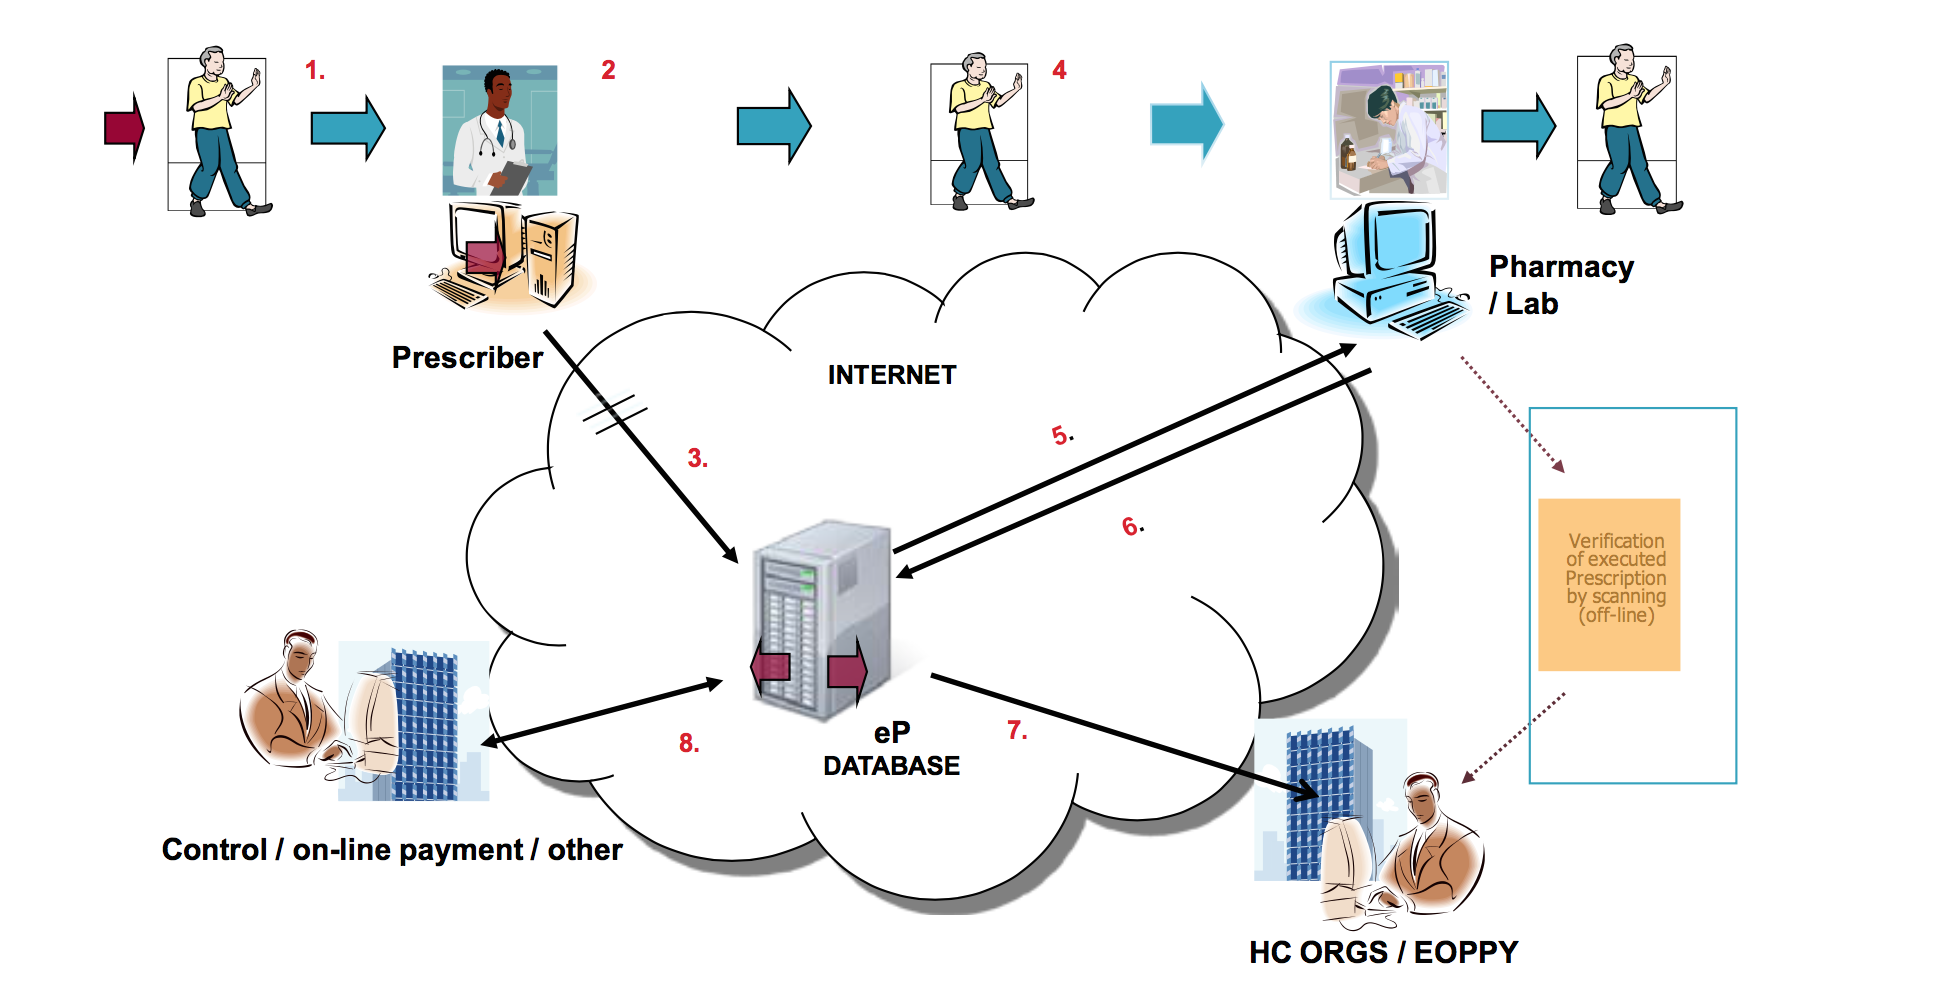
\includegraphics[width=0.7\textwidth]{e-prescr.png}
	    \caption{Το σύστημα E-prescription στην Ελλάδα. }
	    \label{fig:prescr}
	\end{figure}


	

	
	\subsection{Ηλεκτρονικός Ιατρικός Φάκελος (HL7)}
	
	
	
	
	
	
	
	\subsection{epSOS}

\section{Υλοποίηση}
\section{Δοκιμές}
